\section{Problem and test case}
We use Devito~\cite{devito-api,devito-compiler} to solve forward and adjoint
wave equation problems. Devito is a domain-specific language that enables the
rapid development of finite-difference solvers from a high-level description
of partial differential equations. The simplest version of the seismic wave
equation is the acoustic isotropic wave equation defined as:
\begin{equation}
m(x)\frac{\partial^2 u(t, x)}{\partial t^2} - \Laplace u(t, x) = q(t, x),
\label{eqn:wave}
\end{equation}
where $m(x) = \frac{1}{c^2(x)}$ is the squared slowness, $c(x)$ the spatially
dependent speed of sound, $u(t, x)$ is the pressure wavefield, $\Laplace u(t, x)$ denotes the laplacian of the wavefield and $q(t, x)$ is a source term.
Some of our experiments in Section \ref{sec:results} are performed using a more accurate
and more complex version of this equation called Tilted Transverse Isotropy
(TTI)~\cite{zhang2011stable} that takes into account the anisotopic propagation of waves in the earth subsurface (directional dependency of the speed of sound). We leave the TTI equations out of this paper
for brevity. 

The solution to equation~\ref{eqn:wave} forms the forward problem. The seismic inversion problem minimizes the misfit between simulated and observed signal given by:
\begin{equation}
\min_{m} \phi_s(m) = \frac{1}{2} \left\lVert d_{sim} - d_{obs} \right\rVert_2^2.
\end{equation}

This optimization problem is usually solved using gradient based methods such as steepest descent,
where the gradient is computed using the adjoint-state method that involves
the data-flow pattern from Figure \ref{fig:dataflow}.

The values of $m(x)$ used in this work are derived from the Overthrust
model~\cite{aminzadeh1996three} over a grid of $287 \times 881 \times
881$ points, including an absorbing layer of 40 points on each
side. The grid spacing is $25m$ in space. The propagation time is
$4sec$ that corresponds to 2500 timesteps. The wave field at the final
time is shown in Figure~\ref{fig:uncompressed}. The uncompressed size
of this single time step field is just under 900MB. If one were to
store all the timesteps, this would require 2.3TB of memory.

\begin{figure}
\begin{center}
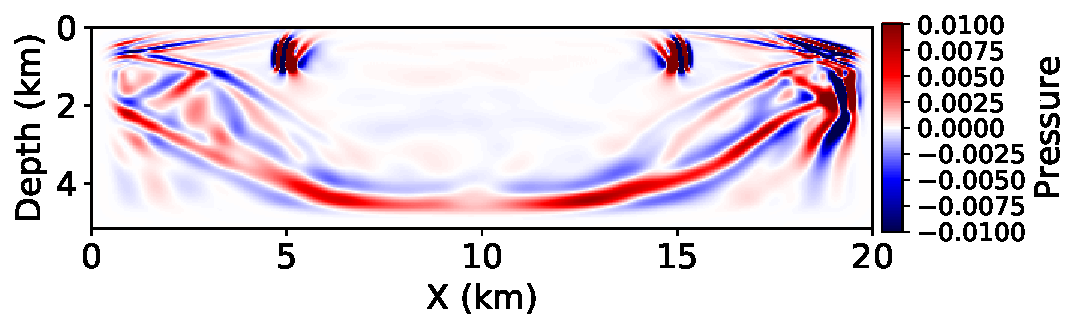
\includegraphics[width=0.8\linewidth]{images/uncompressed.pdf}
\end{center}
\caption{Cross-section of the wavefield used as a reference sample for
  compression and decompression. This field was formed after a Ricker
  wavelet source was placed at the surface of the model and the wave propagated for 2500
  timesteps. This is a vertical (x-z) cross-section of a 3D field, taken at
  the $y$ source location}
\label{fig:uncompressed}
\end{figure}

To implement Revolve with Devito, we use pyRevolve~\cite{kukreja2018high} which
is a python library to manage the execution of checkpointed adjoint computations. The performance model in
section~\ref{sec:performance_model} assumes that the implementation is similar
to pyRevolve, which stores a checkpoint by copying a portion of the operator's
working memory to the checkpointing memory and similarly loads a checkpoint by
copying from the checkpointing memory to the operator's working memory. Although
a perfect implementation of checkpointing may be able to avoid these copies, the
overhead attached to these copies can be ignored for an operator that is
sufficiently computationally intensive. However, we include the overheads in the
model to verify this assumption. 

For benchmarking we used a dual-socket
Intel(R) Xeon(R) Platinum 8180M @ 2.50 Ghz (28 cores each), henceforth
called Skylake. 